\documentclass[tikz]{standalone}

\usetikzlibrary{arrows,shadows,positioning,fit}

\begin{document}

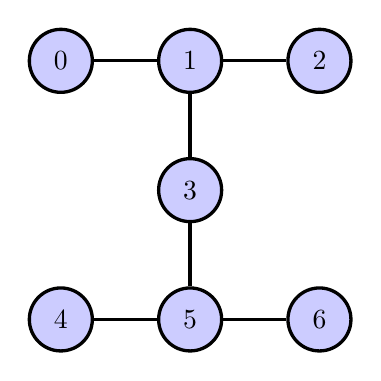
\begin{tikzpicture}
    \tikzset{
        node/.style={
                very thick,
                circle,
                fill=blue!20,
                draw,
                minimum size=.8cm,
            }
    }
    \node[node] (0) {$0$};
    \node[node] (1) [right = .8cm of 0] {$1$};
    \node[node] (2) [right = .8cm of 1] {$2$};
    \node[node] (3) [below = .8cm of 1] {$3$};
    \node[node] (5) [below = .8cm of 3] {$5$};
    \node[node] (4) [left  = .8cm of 5] {$4$};
    \node[node] (6) [right = .8cm of 5] {$6$};

    \path[draw, very thick]
    (0) edge node {} (1)
    (1) edge node {} (2)
    (1) edge node {} (3)
    (3) edge node {} (5)
    (5) edge node {} (4)
    (5) edge node {} (6);
\end{tikzpicture}

\end{document}